\section{Referencia de la Clase Busqueda\-Almacen}
\label{classBusquedaAlmacen}\index{BusquedaAlmacen@{BusquedaAlmacen}}
Clase que sirve para seleccionar un almac\'{e}n.  


{\tt \#include $<$busquedaalmacen.h$>$}

Diagrama de colaboraci\'{o}n para Busqueda\-Almacen:\begin{figure}[H]
\begin{center}
\leavevmode
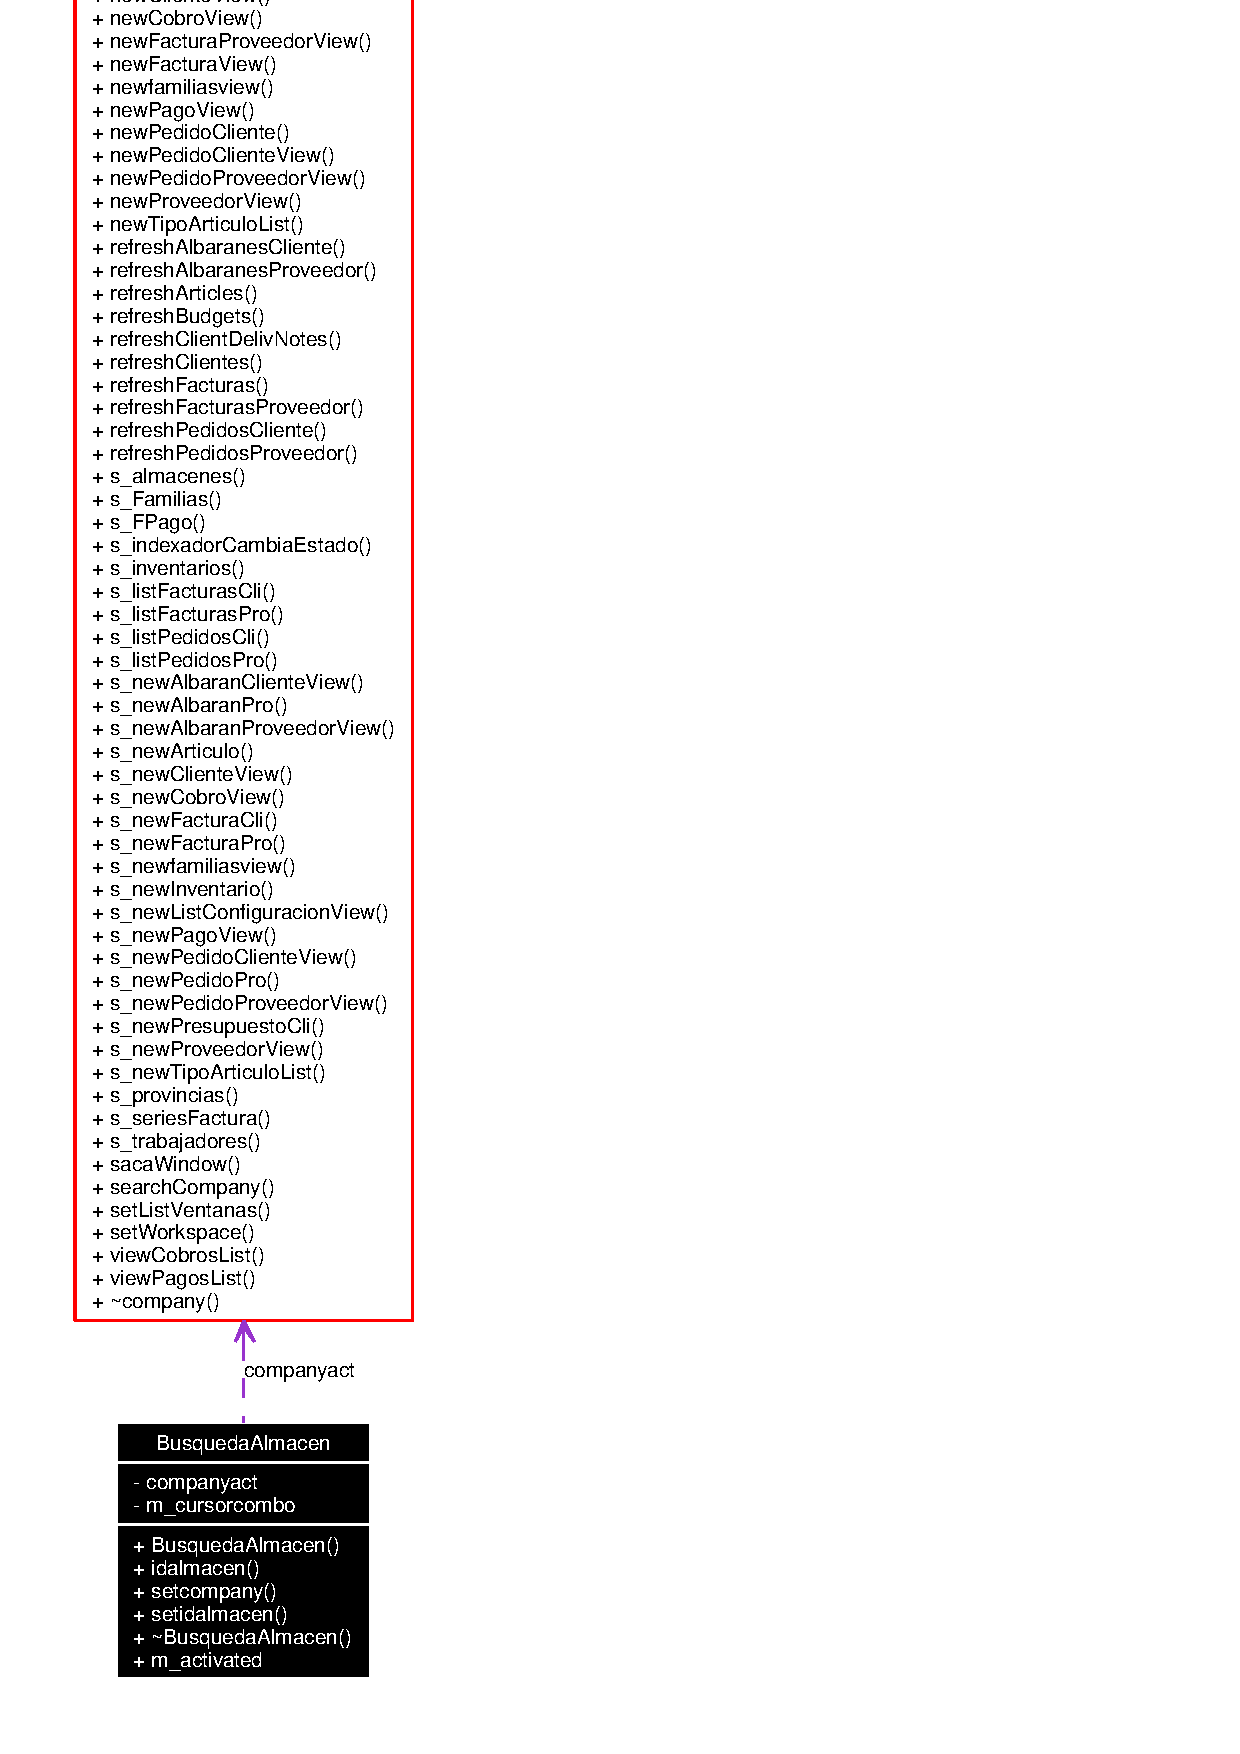
\includegraphics[width=99pt]{classBusquedaAlmacen__coll__graph}
\end{center}
\end{figure}
\subsection*{Slots p\'{u}blicos}
\begin{CompactItemize}
\item 
void {\bf m\_\-activated} (int index)\label{classBusquedaAlmacen_i0}

\end{CompactItemize}
\subsection*{Se\~{n}ales}
\begin{CompactItemize}
\item 
void {\bf value\-Changed} (QString)\label{classBusquedaAlmacen_l0}

\end{CompactItemize}
\subsection*{M\'{e}todos p\'{u}blicos}
\begin{CompactItemize}
\item 
{\bf Busqueda\-Almacen} (QWidget $\ast$parent=0, const char $\ast$name=0)\label{classBusquedaAlmacen_a0}

\item 
QString {\bf idalmacen} ()\label{classBusquedaAlmacen_a1}

\item 
void {\bf setcompany} ({\bf company} $\ast$comp)\label{classBusquedaAlmacen_a2}

\item 
virtual void {\bf setidalmacen} (QString idalmacen)\label{classBusquedaAlmacen_a3}

\end{CompactItemize}


\subsection{Descripci\'{o}n detallada}
Clase que sirve para seleccionar un almac\'{e}n. 

Creamos un QCombo\-Box que sirve para presentar la lista de almacenes disponibles para poder seleccionar uno de ellos. 



La documentaci\'{o}n para esta clase fu\'{e} generada a partir de los siguientes archivos:\begin{CompactItemize}
\item 
busquedaalmacen.h\item 
busquedaalmacen.cpp\end{CompactItemize}
